% !TeX spellcheck = cs_CZ
\wikitextrule
\begin{example}\label{mai:exam065}
  \textbf{Bernoulliovo (binomické) rozdělení}\newline\small
  Představme si opět Bernoulliův pokus o \(n\) opakováních a pravděpodobností zdaru při jednom 
  opakování rovnou \(p\) (příklad \ref{mai:exam057}). Náhodnou veličinu \(X\) definujme jako počet 
  zdarů při tomto pokusu. Táto veličina nabývá všech celočíselných hodnot \(x_j = j, 0 \leq j \leq 
  n\), přitom hodnoty \(j\) nabývá s pravděpodobností určenou vztahem (\ref{mai:eq055}), v němž za 
  \(x\) dosadíme \(j\). 
  
  {\centering
   \captionsetup{type=figure}
   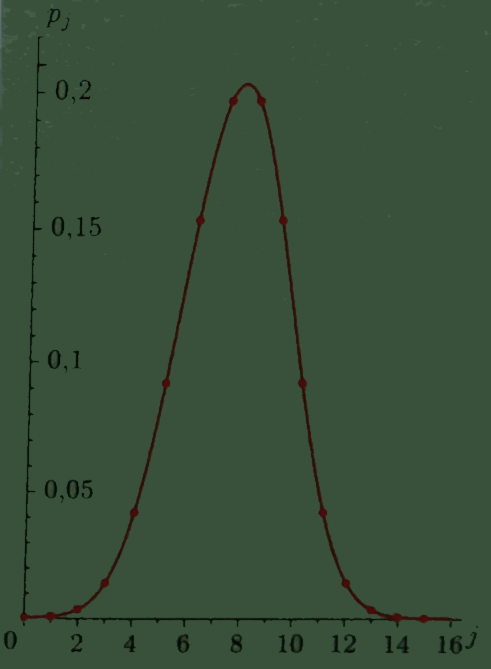
\includegraphics[width=0.4\linewidth]{mai_fig044.png}
   \captionof{figure}{Bernoulliovo rozdělení
   \cite[s.~229]{Musilova2009MA1}
   \label{mai:fig044}}
  \par}
  
  Získané rozdělení je tedy
  \begin{equation*}
    \lbrace j,p_j\rbrace, \qquad\text{kde}\qquad p_j = 
      \begin{pmatrix} n \\ j \end{pmatrix}p_j(1 - p)^{n-j}.
  \end{equation*}
  Graf Bernoulliova rozdělení, které je často nazýváno také binomickým, je na obrázku 
  \ref{mai:fig044} pro \(n = 15\) a \(p = 1/2\).
  
  Z grafu je názorně vidět, co to znamená, že některé hodnoty veličiny \(X\) jsou více a jiné méně 
  pravděpodobné. Hodnota \(x_i\), veličiny \(X\), které odpovídá největší pravděpodobnost \(p_i\), 
  se nazývá nejpravděpodobnější hodnota. V případě Bernoulliova rozdělení na obrázku 
  \ref{mai:fig044} jsou takové hodnoty dvě, konkrétně \(x_7 = 7\) a \(x_8 = 8\).
\normalsize
\end{example}